%!TEX root = "../../DA_GUI.tex"

%	--------------------------------------------------------
% 	Aufbau der Benutzeroberfläche
%	--------------------------------------------------------

\chapter{Elemente der Benutzeroberfläche}
In diesem Kapitel wird der grundlegende Aufbau aller Fenster und Benutzeroberflächen von C Compact beschrieben - sowohl die konzeptuelle Konstruktion als auch die Implementierung.
\section{Das Konzept}
Die Erscheinung und Bedienung von C Compact folgt durchgehend der grundlegenden Idee, eine einfach und intuitiv zu bedienende Entwichlungsumgebung zu schaffen. Das bedeutet, Features möglichst Zielgruppenorientiert zu integrieren und überflüssige Funktionen zu vermeiden. Durch besondere Rücksicht auf Vollständigkeit und logische Bedienvorgänge haben wir ein durchgängig logisches Bedienerlebnis angestrebt.
Konkret haben wir uns dabei an folgende Ŕegeln gehalten:
\begin{itemize}
\item Das Erscheinen von Elementen in der Benutzeroberfläche soll logisch begründbar und verständlich vermittelbar sein
\item Funktionen, die im FSST-Unterricht der ersten und zweiten Klassen wahrscheinlich nicht benötigt werden, werden vermieden oder sind standardmäßig deaktiviert; Bedienelemente werden also auf das wesentlichste reduziert
\item Wir sind der Meinung, dass eine intuitiv zu bedinenede Oberfläche nicht durch Animationen und große Symbole erzeilt werden kann, sondern durch einfache, bereits bekannte Konzepte. So sind in C Compact bekannte Elemente wie beispielsweise eine Menüleiste mit gewohnten Datei- und Dokumentoperationen zu finden (Siehe Kapitel \ref{sec:gui-main-menu}).
%TODO reference GUImain
\end{itemize}

\subsection{Daraus resultierende Einschränkungen}
Durch diese Reduktion der gesamten Oberfläche ist C Compact auf einen bestimmten Zweck, also die Ausbildung, beschränkt. Das sehen wir allerdings nicht als Nachteil, sondern als besondere Stärke. Mit C Compact wollen wir eine Entwicklungsumgebung schaffen, die Anfänger nicht überfordert und ihnen hilft, sich auf das wesentliche zu konzentrieren.
Das Konzept einer anfängerfreundlichen Entwichlungsumgebung ist mit dem Aufbau einer Umgebung für die professionelle Entwicklung nicht vereinbar. C Compact soll aber auf späteres Arbeiten mit komplexeren Programmen vorbereiten. Schüler, die ihre erste Programmiersprache mit C Compact erlernen, kennen bereits den Umgang mit einem Debugger und haben ein tieferes verständnis für den Ablauf von Programmen.

%TODO add window desc. for launcher, quest seleter, package selecter
\section{Elemente und Fenster Der Benutzeroberfläche}
Neben dem Hauptfenster, das den Kern der Benutzeroberfläche darstellt, gibt es eine Reihe von kleineren Aktionsfenster, Dialogen und Einstellungsfenstern, die zum reibungslosen Ablauf bei der Bedienung von C Comapct beitragen. Das Hauptfenster selbst wird in Kapitel \ref{sec:gui-main} beschrieben.

\subsection{Launcher}
...

\subsection{Einstellung der Sprache}
Wenn C Compact zum ersten Mal gestartet wird, wird zu allererst dieses fenster angezeigt. Der Benutzer wird gebeten, eine Sprache zu wählen. Später kann die Sprache über das Menü ,,Datei'' im Hauptfenster (Siehe Kapitel \ref{sec:gui-main-menu-file}) geändert werden. Die Änderungen werden erst wirksam, wenn der Benutzer die neue Sprache mit ,,OK'' bestätigt. Dann wird C Compact neu gestartet.
%TODO ref translations, Sprache

\begin{figure}[htp]
\centering
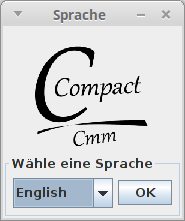
\includegraphics[width=0.3\textwidth]{./media/images/gui/elements/Bildschirmfoto-Sprache.png}
\caption{Auswahl der Sprache}
\label{fig:win-lang}
\end{figure}

Dieses Fenster ist in der Klasse \textbf{GUILanguage} im Package \textbf{at.jku.ssw.cmm.gui.properties} implementiert. 

\subsection{Allgemeine Einstellungen}
Dieses fenster enthält allgemeine Optionen zum Haupfenster der Benutzeroberfläche.
%TODO TODO TODO hier weitermachen

%TODO ref GUImainSettings

